\chapter{Serverless design patterns} \label{cha:patterns}

In this chapter we take a look at serverless design patterns. Design patterns describe commonly accepted, reusable solutions to recurring problems \parencite{hohpe2004enterprise}. A design pattern is not a one-size-fits-all solution directly translatable into software code, but rather a formalized best practice that presents a common problem in its context along a general arrangement of elements that solves it \parencite{gamma94designPatterns}. The patterns in this chapter are sourced from scientific literature on serverless computing as well as cloud provider documentation \parencite[][]{aws18serverlessLens, microsoft18cloudPatterns}. Literature on object-oriented patterns (OOP) \parencite{gamma94designPatterns}, SOA patterns \parencite{rotem12soa}, cloud design patterns \parencite{microsoft18cloudPatterns} as well as enterprise integration patterns (EIP) \parencite{hohpe2004enterprise} was also reviewed for applicable practices.

The patterns are grouped into four categories for better readability. How the patterns fit together is sketched out in figure \ref{fig:patternLanguage}. These interrelations form a \textit{pattern language}, i.e. a structural organization of pattern relations \parencite{rotem12soa}.

\begin{figure}[h]
  \begin{center}
    \makebox[\textwidth]{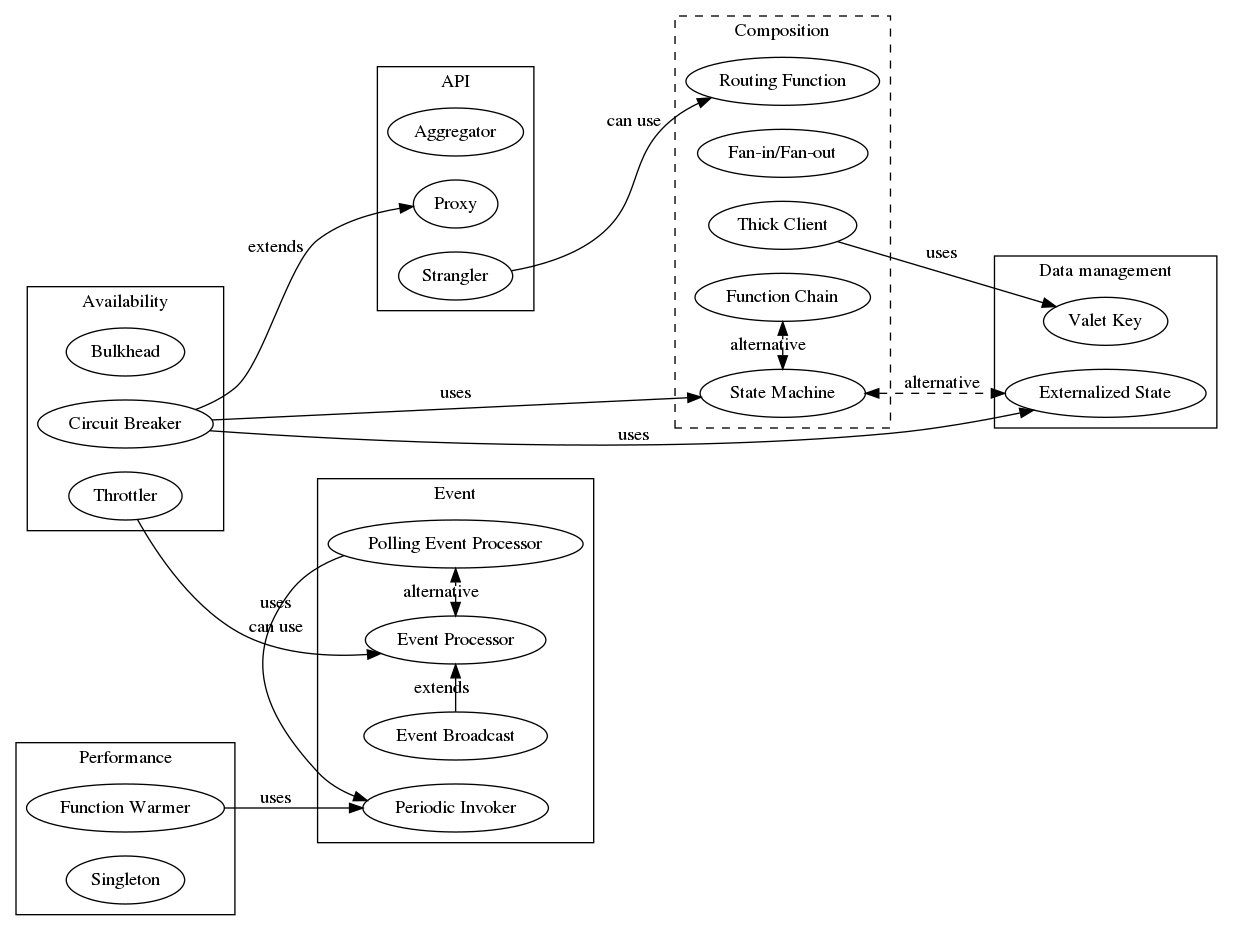
\includegraphics[width=0.9\paperwidth]{pattern-language.png}}
  \end{center}
  % 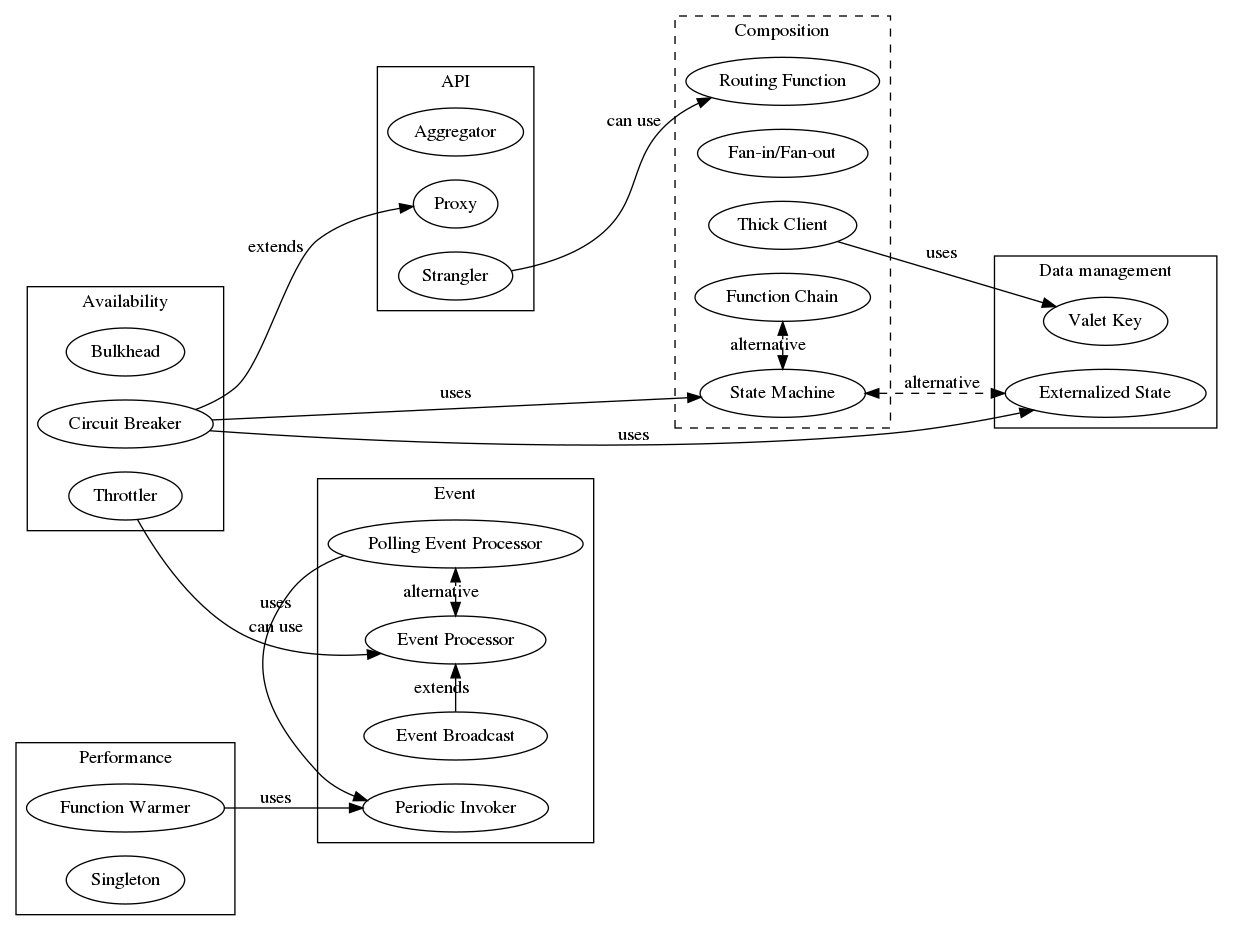
\includegraphics[width=1.1\textwidth]{pattern-language.pdf}
  % \centering
  \caption{Pattern language}
  \label{fig:patternLanguage}
\end{figure}

\section{Composition patterns} \label{sec:compositionPatterns}

How to compose and orchestrate serverless functions together into more expansive sequences or workflows?

\subsection{Routing Function} \label{subsec:routingFunction}

\textbf{Problem:} How to branch out execution flow based on request payload?

\begin{figure}[h]
  \centering
  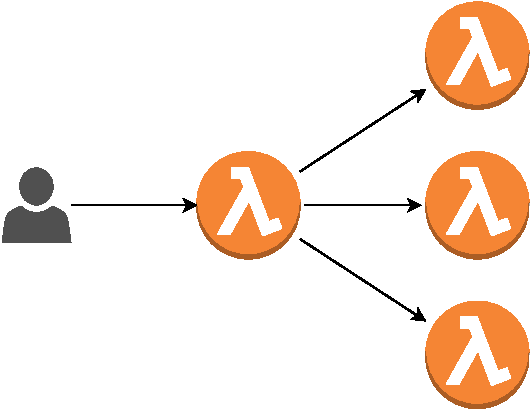
\includegraphics[width=0.4\textwidth]{patterns/routing-function.pdf}
  \caption{Routing Function}
  \label{fig:patternRoutingFunction}
\end{figure}

\textbf{Solution:} Use a central routing function to receive requests and invoke appropriate functions based on request payload.

This pattern involves instantiating a routing function that contains all the necessary information to route requests to other functions. All function invocations are directed to the routing function, which in turn invokes target functions according to request payload. The routing function finally passes target function return value over to the client.

It's notable that FaaS platforms commonly provide API gateways and other tools for routing, for example the Amazon API Gateway \parencite{awslambda0218}. These tools however are mostly limited to path-based routing, whereas a routing function can be implemented to support more dynamic use cases. Also notably, according to an industry survey \parencite{leitner18industrialpractice}, some practitioners opted for the Routing Function pattern over platform API gateway services as they found the latter cumbersome to manage. \textcite{sbarski2017serverless} similarly postulate that the pattern ``can simplify the API Gateway implementation, because you may not want or need to create a RESTful URI for every type of request''. One advantage of the pattern is that the routing function can be used to supplement request payload with additional context or metadata. A centralized routing function also means that all routing configuration is found in one place, and that public-facing API routes only need to be configured for one function, not all of them \parencite{leitner18industrialpractice}. From a client's point of view, the Routing Function has the benefit of abstracting backend services so that calls can be rerouted to different services without changing client implementation; this can be put to use for example in A/B testing by partially rolling out new updates to selected clients \parencite{microsoft18cloudPatterns}.

The pattern's major disadvantage is double billing, as the routing function essentially has to block and wait until the target function finishes execution. Additionally, as routing is implemented at function code level, information about function control flow gets hidden in implementation rather than being accessible from configuration \parencite{leitner18industrialpractice}. Also, like any centralized service, the Routing Function can potentially introduce a single point of failure or a performance bottleneck \parencite{microsoft18cloudPatterns}.

The Routing Function resembles the OOP Command pattern which is used to decouple caller of the operation from the entity that carries out the processing via an intermediary command object \parencite{gamma94designPatterns}. A related EIP pattern is the Content-Based Router, which ``examines the message content and routes the message onto a different channel based on data contained in the message'' \parencite{hohpe2004enterprise}. Also pertinent to the serverless Routing Function, \textcite{hohpe2004enterprise} caution that the Content-Based Router should be made easy to maintain as it can become a point of frequent configuration. Finally, Microsoft's cloud design patterns includes the Gateway Routing pattern that's similarly employed to ``route requests to multiple services using a single endpoint'' \parencite{microsoft18cloudPatterns}.

\subsection{Function Chain} \label{subsec:functionChain}

\textbf{Problem:} Task exceeds maximum function execution duration, resulting in a timeout.

\begin{figure}[h]
  \centering
  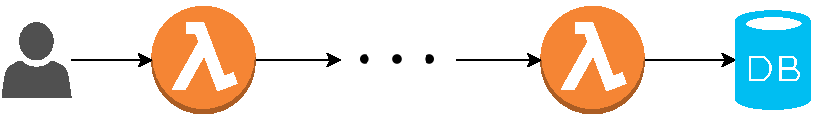
\includegraphics[width=0.6\textwidth]{patterns/function-chain.pdf}
  \caption{Function Chain}
  \label{fig:patternFunctionChain}
\end{figure}

\textbf{Solution:} Split the task into separate function invocations that are chained together sequentially.

The Function Chain comprises of an initial function invocation and any number of subsequent invocations. The initial function begins computation while keeping track of remaining execution time. For example in AWS Lambda the execution context contains information on how many milliseconds are left before termination \parencite{awslambda0218}. Upon reaching its duration limit, the initial function invokes another function asynchronously, passing along as parameters any state necessary to continue task computation. Since the intermediary invocation is asynchronous (``fire-and-forget''), the initial function can terminate without affecting the next function in chain.

The Function Chain pattern is in effect a workaround over the duration limit that FaaS platforms place on function execution \parencite{leitner18industrialpractice}. The pattern was reported to be used at least occasionally in an industry study by \textcite{leitner18industrialpractice}. Its disadvantages include strong coupling between chained functions, increase in the number of deployment units and the overhead of transferring intermediate execution state and parameters between each chained function. \textcite{leitner18industrialpractice} also note that splitting some types of tasks into multiple functions can be difficult. Finally, as the pattern relies on asynchronous invocation, the last function in chain has to persist computation result into an external storage for the client to access it which brings in further dependencies.

\subsection{Fan-out/Fan-in} \label{subsec:FanoutFanin}

\textbf{Problem:} Resource limits on a single function lead to reduced throughput.

\begin{figure}[h]
  \centering
  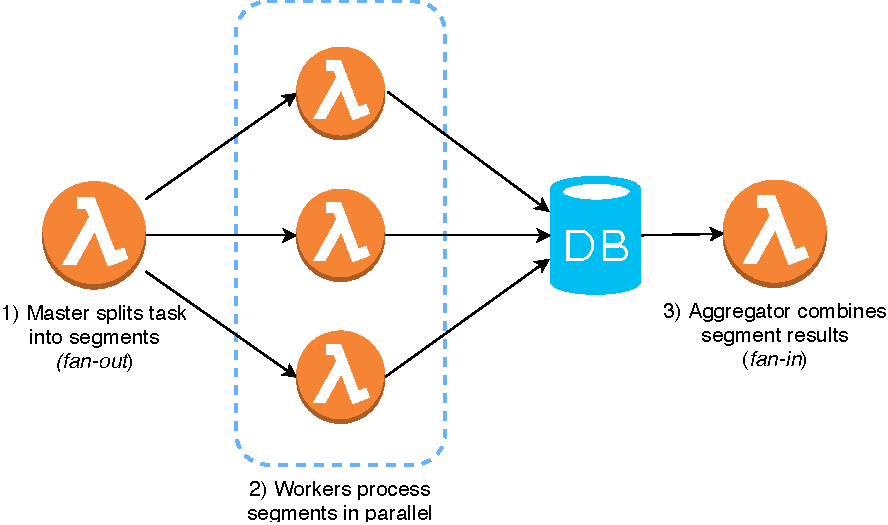
\includegraphics[width=0.75\textwidth]{patterns/fan-out-fan-in.pdf}
  \caption{Fan-out/Fan-in}
  \label{fig:fantOutFanIn}
\end{figure}

\textbf{Solution:} Split task into multiple parallel invocations.

As discussed above, serverless functions are limited both in execution duration as well as CPU and memory capacity. The Function Chain pattern (section \ref{subsec:functionChain}) works around the former limitation but is still constrained by a single function's computing resources, which can result in prohibitively slow throughput for compute-intensive tasks. The Fan-out/Fan-in pattern is an alternative approach that takes advantage of serverless platforms' inherent parallelism. The pattern consists of a master function that splits the task into segments and then asynchronously invokes a worker function for each segment. Having finished processing, each worker function stores its result on a persistence layer, and finally an aggregator function combines the worker results into a single output value -- although the aggregation step can be omitted in cases where intermediary results suffice. As each worker function invocation runs in parallel with its own set of resources, the pattern leads to faster completion of the overall task. \parencite{zambrano18patterns}

The Fan-out/Fan-in pattern lends itself well to tasks that are easily divisible into independent parts: the efficiency gained depends on the granularity of each subdivision. Conversely, an apparent limitation to the pattern is that not all tasks can be easily distributed into separate worker functions. \textcite{mcgrath16cloudEventParadigms} utilize the pattern in ``easily and performantly solving a large-scale image resizing task''. The authors point out how the pattern reduces development and infrastructure costs compared to a traditional multi-threaded application which ``typically demands the implementation of a queueing mechanism or some form of worker pool''. \textcite{lavoie19efficiency} similarly study ``the efficiency of a serverless architecture for running highly parallelizable tasks'' in comparison to a conventional MapReduce solution running on Apache Spark, concluding that ``the serverless technique achieves comparable performance in terms of compute time and cost''.

\textcite{hohpe2004enterprise} present a similar approach to messaging with the EIP pattern of Composed Message Processor, which ``splits the message up, routes the sub-messages to the appropriate destinations and re-aggregates the responses back into a single message.''

\subsection{Externalized State} \label{subsec:externalizedState}

\textbf{Problem:} How to share state between sequential or parallel serverless function instances?

\begin{figure}[h]
  \centering
  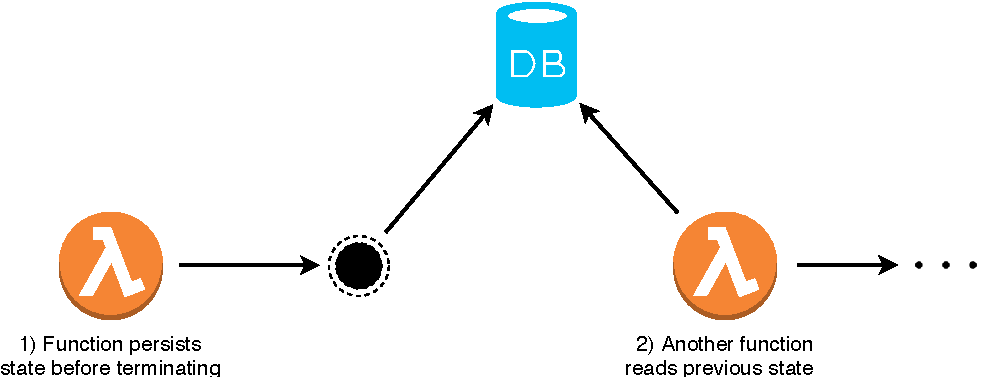
\includegraphics[width=0.8\textwidth]{patterns/externalized-state.pdf}
  \caption{Externalized State}
  \label{fig:externalizedState}
\end{figure}

\textbf{Solution:} Store function state in external storage.

Serverless functions are, as discussed, stateless by design. Function instances are spawned and terminated ephemerally in a way that an instance has no access to any preceding or parallel instance state. Not all serverless use cases are purely stateless however, so being able to store and share state between function instances comes up as a common requirement. This is evidenced by a survey on serverless adoption in which two thirds of respondents reported at least sometimes applying the Externalized State pattern, making it by far the most common among the surveyed patterns \parencite{leitner18industrialpractice}.

The Externalized State pattern is a fundamental pattern that consists of storing a function's internal state in external storage such as a database or a key-value store. The pattern is used to reliably persist state between sequential function invocations, and on the other hand to share state between parallel invocations. Imposing state on a stateless paradigm doesn't come free though, as relying on external storage induces latency and extra programming effort as well as the operational overhead of managing a storage component. \parencite{leitner18industrialpractice}

\subsection{State Machine} \label{subsec:stateMachine}

\textbf{Problem:} How to coordinate complex, stateful procedures with branching steps?

\begin{figure}[h]
  \centering
  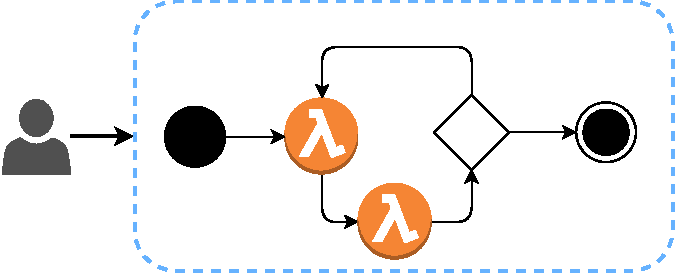
\includegraphics[width=0.55\textwidth]{patterns/state-machine.pdf}
  \caption{State Machine}
  \label{fig:patternStateMachine}
\end{figure}

\textbf{Solution:} Split a task into a number of discrete functions and coordinate their execution with an orchestration tool.

\textcite{hong18securingviaserverlesspatterns} describe the State Machine pattern as ``building a complex, stateful procedure by coordinating a collection of discrete Lambda functions using a tool such as AWS Step Functions''. These orchestration tools consist of a collection of workflow states and transitions between them, with each state having its associated function and event sources -- essentially a serverless a state machine \parencite{cncf18serverlessWG}. Figure \ref{fig:patternStateMachine} could for example represent a workflow where the first function attempts a database insert, the second function checks whether the operation succeeded, and depending on the result either the operation is retried or execution is finished. The advantage of using provider tooling for workflow execution is that there's no need for external storage as the orchestrator keeps track of workflow state. Downsides on the other hand include extra cost arising from orchestration tooling as well as the overhead of managing workflow descriptions.

\textcite{lopez18orchestration} compare three major FaaS orchestration systems: AWS Step Functions, IBM Composer and Azure Durable Functions. The compared systems typically support function chaining, conditional branching, retries and parallel execution, with workflows defined either in a Domain-Specific Language or directly in code. One restriction in Amazon's orchestrator is that a composition cannot be synchronously invoked and is thus not composable in itself: a state machine cannot contain another state machine. AWS Step Functions was also the least programmable among the compared systems, but on the other hand the most mature and performant. Finally, the authors observe that none of the provider-managed orchestration systems are prepared for parallel programming, with considerable overheads in concurrent invocation.

A SOA pattern analogous to the State Machine is the Orchestrator, in which ``an external workflow engine activates a sequence (simple or compound) of services to provide a complete business service''. The Orchestrator aims to keep business processes agile and adaptable by externalizing them from service implementations: instead of hard-coding service interactions they are defined, edited and executed within a workflow engine. Used properly, the Orchestrator can add a lot of flexibility to the system. Difficulty however lies in implementing services as composable and reusable workflow steps while still keeping them useful as autonomous services. \parencite{rotem12soa}.

\subsection{Thick Client} \label{subsec:thickClient}

\textbf{Problem:} Routing client-service requests through an intermediary server layer causes extra costs and latency.

\begin{figure}[h]
  \centering
  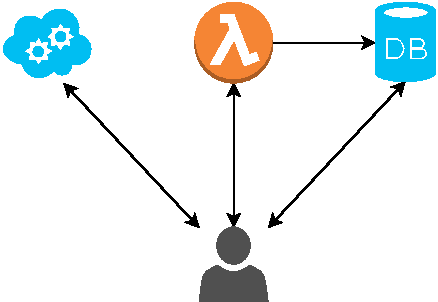
\includegraphics[width=0.4\textwidth]{patterns/thick-client.pdf}
  \caption{Thick Client}
  \label{fig:patternThickClient}
\end{figure}

\textbf{Solution:} Create thicker, more powerful clients that directly access services and orchestrate workflows.

Serverless applications, as described in chapter \ref{cha:serverless}, typically rely heavily on third-party cloud services (BaaS) interspersed with custom logic in form of FaaS functions. In a traditional three-tier web application architecture interaction with these external services would be handled by a server application that sits between client and service layers \parencite{robert2016serverlessarchitectures}. Following this model, the client can be limited in functionality whereas the server application plays a larger role. \textcite{sbarski2017serverless} point out that the model of the backend as a gatekeeper between client and services is in conflict with the serverless paradigm. First of all, using FaaS as a middle layer in front of cloud resources directly translates into extra costs: on top of paying for the cloud service call, one has to pay for function invocation and execution for the duration of the network call as well as data transfer between the service and the FaaS provider. Secondly, a middle layer of FaaS results in extra network hops which increases latency and reduces user experience. The authors thus advise against routing everything through a FaaS layer, and advocate building thick clients that communicate directly with cloud services and orchestrate workflows between them.

In addition to improving cost and network efficiency, the Thick Client has the advantage of improved changeability and separation of concerns, as the single monolithic backend application is replaced by more isolated and self-contained components. Doing away with the central arbiter of a server application does come with its trade-offs, including a need for distributed monitoring and further reliance on the security of third-party services. Importantly not all functionality can or should be moved to the client: security, performance or consistency requirements among others can necessitate a server-side implementation. \parencite{robert2016serverlessarchitectures}.

The Thick Client pattern depends on fine-grained, distributed, request-level authentication in lieu of a gatekeeper server application. This follows naturally from the way serverless functions operate: being stateless and continuously scaling up and down, maintaining a session between the backend and the cloud services is infeasible. Instead of automatically trusting all requests originating from the backend, each cloud service request has to be individually authorized. From a cloud service's point of view, requests originating from a serverless function or directly from the client are both equally untrusted. Hence in serverless architectures, skipping the backend layer is preferable whenever a direct connection between client and services is possible. The Valet Key pattern in section \ref{subsec:valetKey} describes one example of a request-level authentication mechanism. \parencite{adzic2017serverless}

\section{Event patterns} \label{sec:eventPatterns}

How to handle asynchronous workflows triggered by external events?

\subsection{Event Processor} \label{subsec:Eventprocessing}

\textbf{Problem:} How to execute a task on-demand upon event occurrence?

\begin{figure}[h]
  \centering
  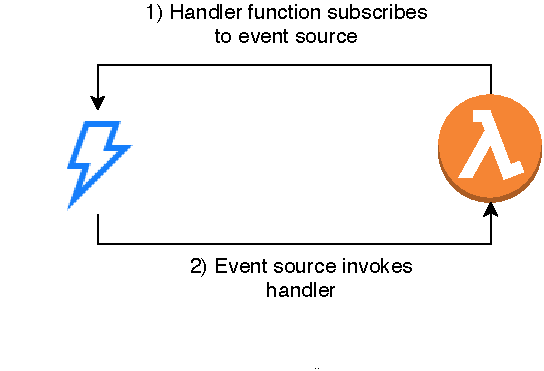
\includegraphics[width=0.45\textwidth]{patterns/event-processor.pdf}
  \caption{Event Processor}
  \label{fig:patternEventProcessor}
\end{figure}

\textbf{Solution:} Subscribe a serverless function to a cloud event such as file upload or database change.

The Event Processor pattern consists of subscribing a serverless function to a cloud event source so that when the event occurs, the subscribed function gets invoked with access to the event context \parencite{hong18securingviaserverlesspatterns}. Serverless platforms typically offer a number of integration points to events that originate from platform services. An AWS Lambda function, for example, can be triggered by file uploads, database change events, message queue and notification services, IoT events and others \parencite{awslambda0218}.

\textcite{baldini17currentTrends} mention thumbnail generation triggered by image upload as an exemplary use case of serverless event processing: a bursty, compute-intensive task triggered on-demand by a cloud event. A traditional approach would be to implement a poller system that regularly checks for new images and generates thumbnails as images are detected. Such a system would require constant operation, and depending on polling interval the design leads to either extra network traffic or potentially long delay between event occurrence and processing. The design is especially wasteful in cases where new images come in infrequently. The Event Processor pattern, in turn, can bring considerable cost benefit in case of infrequent or irregular workflows as computation is only ran when necessary \parencite{hong18securingviaserverlesspatterns}. Another advantage is scalability, as functions are automatically invoked as per the number of events: a large number of events occurring at once leads to a similarly large number of functions executing in parallel \parencite{hong18securingviaserverlesspatterns}.

The Event Processor has two counterparts among SOA patterns. In terms of scalability, a serverless Event Processor essentially implements the Service Instance pattern which involves ``deploying multiple instances of service business logic'' to address increased service load. Aptly, the Service Instance pattern is ``best suited for stateless service implementations''. Another related SOA pattern is the Inversion of Communications in which services eschew point-to-point communication in favour of event-driven architecture to reduce coupling between event sources and consumers. The pattern's downsides include the added complexity of designing a system as events and the difficulty of debugging complex event chains. \parencite{rotem12soa}

The Event Processor can also be seen as a serverless form of the Event-Driven Consumer EIP pattern: a message consumer that sits dormant with no active threads until invoked by the messaging system. In essence, the pattern bridges the gap between external events and application-specific callbacks. A notable feature of an Event-Driven Consumer is that it automatically consumes messages as soon as they become available, which in effect means that the consumer has no control on its consumption rate: see the Polling Event Processor in section \ref{subsec:PollingEventProcessor} for an alternative solution. \parencite{hohpe2004enterprise}

Another point to keep in mind when implementing the Event Processor pattern is that some cloud event sources operate in at-least-once message delivery semantics: due to the highly distributed and eventually consistent nature of cloud platforms, events are guaranteed to be triggered at least once, not exactly once \parencite{awslambda0218}. This means that the triggered serverless function should in effect act idempotently, i.e. multiple executions with the same context should result in identical side effects. \textcite{hohpe2004enterprise} introduce a similar concept with the Idempotent Receiver pattern, a listener that can ``safely receive the same message multiple times''. The authors introduce two primary means for achieving idempotency: either explicit deduplication at the receiving end, or defining message semantics to support idempotency. The first approach calls for keeping track of the messages received thus far and ignoring any duplicates among incoming messages, leaving us with the problem of where and for how long to store the message history. The alternative approach is to design messages themselves in a way that ``resending the message does not impact the system'': for example \textit{set account balance to \$10} instead of \textit{increase account balance by \$1}.

\subsection{Periodic Invoker} \label{subsec:periodicInvocation}

\textbf{Problem:} How to execute a task periodically in predefined intervals?

\begin{figure}[h]
  \centering
  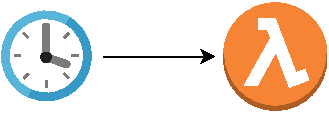
\includegraphics[width=0.35\textwidth]{patterns/periodic-invocation.pdf}
  \caption{Periodic Invoker}
  \label{fig:patternPeriodicInvocation}
\end{figure}

\textbf{Solution:} Subscribe a serverless function to a scheduler.

The Periodic Invoker represents an arrangement where a serverless function is invoked periodically by a scheduler, akin to a cron task in Unix-based systems. First, the scheduler invokes the subscribed function according to its configuration. Second, the function carries out its task. Finally, after execution the function can report execution result out to a notification channel, store it in database or shut down if we're not interested in the outcome. The pattern is both conceptually simple and easy to implement, as all the major serverless providers offer integration to a cloud-based scheduler such as AWS CloudWatch Events \parencite{awslambda0218}. Potential use cases include periodical backups, compliance checks, service health checks, database cleanup tasks and other background jobs that are not latency-critical. \parencite{hong18securingviaserverlesspatterns}

\subsection{Polling Event Processor} \label{subsec:PollingEventProcessor}

\textbf{Problem:} How to react to state change in an external service that doesn't publish events?

\begin{figure}[h]
  \centering
  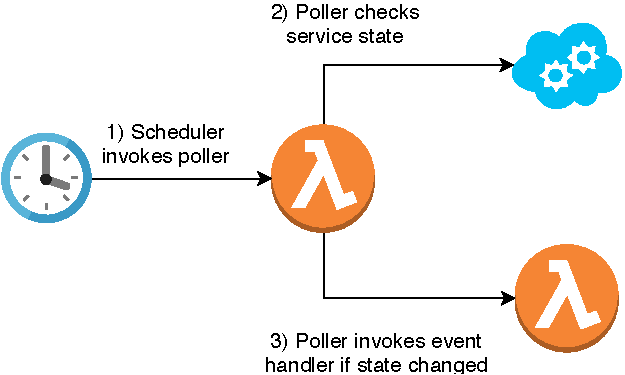
\includegraphics[width=0.55\textwidth]{patterns/polling-event-processor.pdf}
  \caption{Polling Event Processor}
  \label{fig:PollingEventProcessor}
\end{figure}

\textbf{Solution:} Use the Periodic Invoker to actively poll for state changes and trigger events accordingly.

The Event Processor pattern (section \ref{subsec:Eventprocessing}) is used to perform a task in reaction to some state change in another system. The pattern depends on the external system to actively invoke the subscribed function when said state change occurs. Not all systems however are capable of performing such callbacks on state changes, which renders the pattern unusable in some cases. The Polling Event Processor works around this limitation by combining the Event Processor (section \ref{subsec:Eventprocessing}) and Periodic Invoker (section \ref{subsec:periodicInvocation}) patterns to essentially implement an event-driven integration point in front of a service where no such event source originally exists. The pattern consists of a Periodic Invoker that repeatedly checks the state of another service and performs a task when found state matches some condition. The task performed can be either implemented in the polling function itself or separated to another function that the poller invokes.

The Polling Event Processor is equivalent to the EIP pattern of Polling Consumer, where a receiver synchronously polls for a message, processes it and then polls for another. As well as offering eventful integration to non-eventful services, the pattern has the advantage of controlling its consumption rate. Whereas the Event Processor executes tasks as soon as events occur, the Polling Event Processor explicitly polls for new events when it is ready for them. The polling interval can also be configured to implement batching. As a downside, a sparse polling interval leads to increased latency between event occurrence and task execution. On the other hand a more fine-grained polling interval results in wasted resources when there are no events to consume. In short, ``polling enables the client to control the rate of consumption, but wastes resources when there’s nothing to consume.'' \parencite{hohpe2004enterprise}

\subsection{Event Broadcast} \label{subsec:EventBroadcast}

\textbf{Problem:} How to invoke multiple parallel functions as a result of a single event occurrence?

\begin{figure}[h]
  \centering
  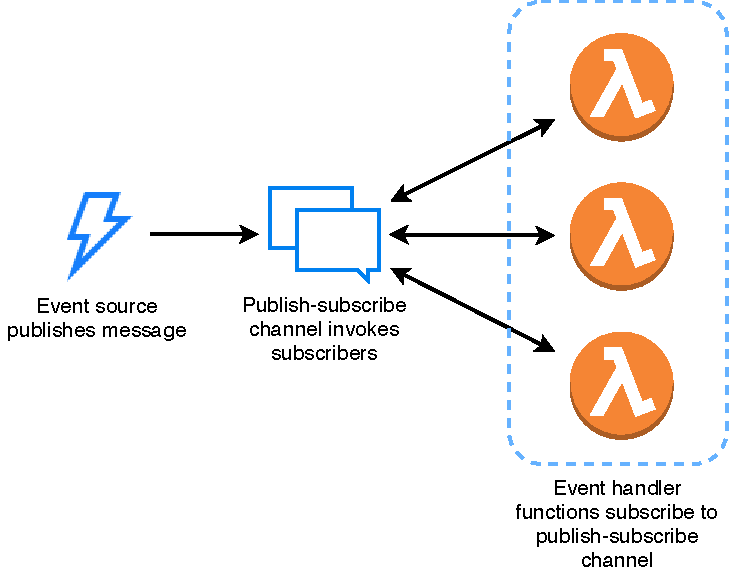
\includegraphics[width=0.6\textwidth]{patterns/event-broadcast.pdf}
  \caption{Event Broadcast}
  \label{fig:eventBroadcast}
\end{figure}

\textbf{Solution:} Subscribe multiple functions to a notification service, publish notification on event occurrence.

The Event Processor pattern (section \ref{subsec:Eventprocessing}) is applicable within cases of 1-to-1 relationship between events and tasks, as exemplified above with image upload triggering thumbnail generation. However in other cases a single event can result in multiple independent tasks. For example the image upload event could as well trigger a database update and a notification email, adding up to three self-contained and parallel tasks. Most event sources only support invoking one function per event which leaves us with a couple of options. First, we could set up a new function that subscribes to the image upload event and in turn asynchronously invokes any number of processor functions, as a sort of a parallel Routing Function \label{subsec:routingFunction}. This approach comes with the operational overhead of needing to set up and maintain an additional function per each event broadcast. An alternative solution is to utilize a publish-subscribe channel such as the AWS Simple Notification Service \parencite{awslambda0218}. The key feature of a publish-subscribe channel is that any number of listeners can subscribe to a single channel, which can be used to overcome the 1-to-1 relationship between event sources and functions. Now instead of subscribing a function directly to an event source, functions subscribe to a message channel that the event source publishes a message to upon event occurrence. In addition to achieving parallel fan-out to multiple functions, the pattern has the added benefit of loosed coupling between event sources and handler functions. \parencite{sbarski2017serverless}

The Event Broadcast's object-oriented counterpart is the Observer: ``define a one-to-many dependency between objects so that when one object changes state, all its dependants are notified and updated automatically'' \parencite{gamma94designPatterns}. Just like above, the pattern decouples observers from the subject; that is, the object that we're interested in publishes its state regardless of the number of interested observers. The EIP pattern of Publish-Subscribe Channel expands the same decoupling to messaging: one input channel is split into multiple output channels, with each subscriber having its own channel and thus receiving its own copy of the original message \parencite{hohpe2004enterprise}.

\section{Integration patterns} \label{sec:integrationPatterns}

How to integrate to external -- including legacy -- systems?

\subsection{Aggregator} \label{subsec:aggregator}

\textbf{Problem:} An operation consists of multiple API requests, resulting in extra network hops between client and service.

\begin{figure}[h]
  \centering
  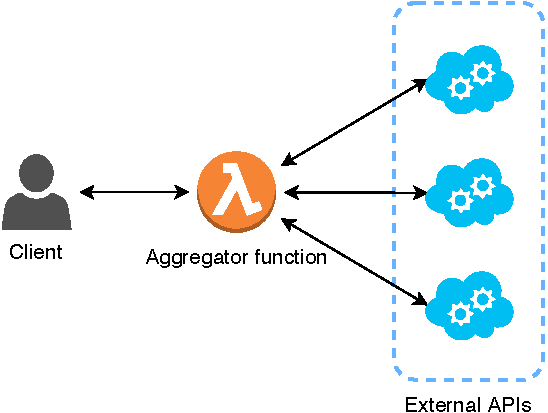
\includegraphics[width=0.5\textwidth]{patterns/aggregator.pdf}
  \caption{Aggregator}
  \label{fig:aggregator}
\end{figure}

\textbf{Solution:} Aggregate multiple API requests under a single serverless function.

Service clients often need to deal with operations that involve performing several API calls, either in parallel or sequentially, and then filtering or combining the results. The operation might utilize multiple different services or just different endpoints of a single service. \textcite{baldini17currentTrends} use the example of combining geolocation, weather and language translation APIs to render a localized weather forecast. Another example concerns a sequential multi-step API call of first fetching an API key, then resource location, and finally performing the actual operation. Composing operations out of multiple cross-service calls is a natural outcome of service oriented architectures, but incurs the penalty of extra resource usage and network latency in clients. The problem is further magnified in microservice and serverless architectures due to the fine service granularity. \parencite{microsoft18cloudPatterns}

The Aggregator pattern consists of wrapping the required API calls into a single serverless function which is then exposed as a singular endpoint to clients. The Aggregator calls each target API and combines the results so that the client is left with a single network call, reducing the risk of network failure. Client resource usage is also reduced since any filtering or aggregation logic is offloaded to the Aggregator. Also ideally the Aggregator function is located near backend services to minimize network latency, and individual API responses are cached whenever possible. \parencite{baldini17currentTrends}

The Aggregator is largely equivalent to the Gateway Aggregation cloud design pattern \parencite{microsoft18cloudPatterns}. \textcite{baldini17currentTrends} in turn split the pattern into API composition and API aggregation, for combined and sequential request flows respectively. It's worth noting that the Aggregator doesn't address the problems of network failure and incomplete requests, as the aggregating function might still encounter failed requests from downstream services. The pattern rather outsources the risk from service consumer to a backend service, working thus opposite to the Thick Client pattern's consumer-driven service orchestration (section \ref{subsec:thickClient}). To ensure reliable operation when one of the API requests fails the Aggregator might internally implement the Compensating Transactions cloud design pattern, i.e. pairing each request with a compensating action that is performed in case of failure \parencite{microsoft18cloudPatterns}. The SOA patterns of Transactional Service and the more heavyweight Saga could also be used to enforce transactional guarantees inside the Aggregator \parencite{rotem12soa}.

\subsection{Proxy} \label{subsec:proxy}

\textbf{Problem:} How to make a legacy service easier to consume for modern clients?

\begin{figure}[h]
  \centering
  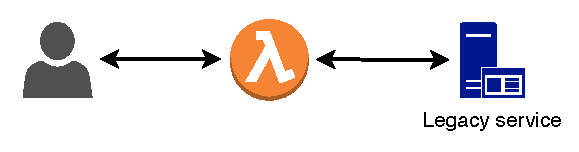
\includegraphics[width=0.5\textwidth]{patterns/proxy.pdf}
  \caption{Proxy}
  \label{fig:proxy}
\end{figure}

\textbf{Solution:} Implement a serverless function as a proxy layer that translates requests between clients and the legacy service.

Applications often need to integrate to a legacy system for some resource or functionality. This requirement might present itself when an outdated but crucial system is in the process of being migrated, or cannot be migrated at all due to reasons of complexity or cost. Legacy systems might suffer from quality issues and use older protocols or data formats, which makes interoperation with modern clients problematic. A client would have to implement support for legacy technologies and semantics, which might adversely affect its own design goals. \parencite{microsoft18cloudPatterns}

The serverless Proxy pattern essentially ``makes legacy services easier to consume for modern clients that may not support older protocols and data formats'' \parencite{sbarski2017serverless}. The pattern consists of a serverless function that acts as a proxy in front of the legacy service, handling any necessary protocol or data format translation and sanity checks. Conversely for client applications, the Proxy offers a clean and modern API for easier consumption. \textcite{sbarski2017serverless} use the example of offering a JSON API in front of a SOAP service. The pattern is also referred to as the Anti-Corruption Layer, alluding to how it works to contain a system's quality issues: ``this layer translates communications between the two systems, allowing one system to remain unchanged while the other can avoid compromising its design and technological approach'' \parencite{microsoft18cloudPatterns}.

\subsection{Strangler} \label{subsec:strangler}

\textbf{Problem:} How to migrate an existing service to serverless architecture in a controlled fashion?

\begin{figure}[h]
  \centering
  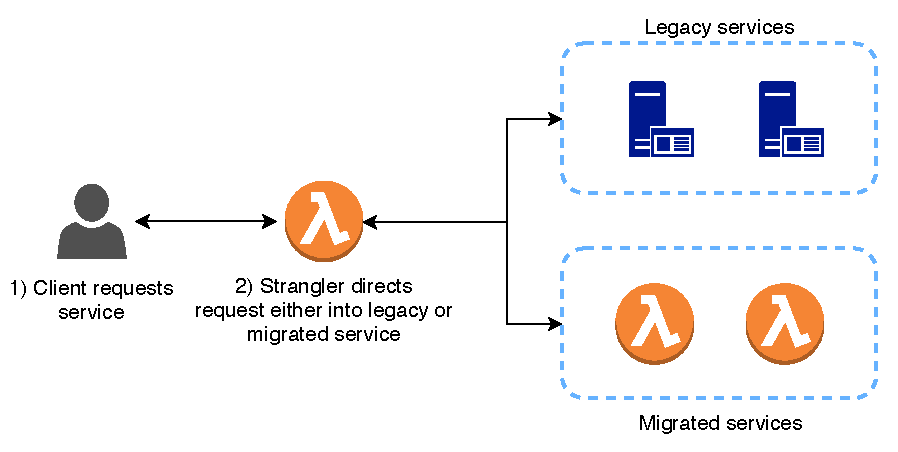
\includegraphics[width=0.75\textwidth]{patterns/strangler.pdf}
  \caption{Strangler}
  \label{fig:strangler}
\end{figure}

\textbf{Solution:} Create a façade in front of the legacy API and incrementally replace individual routes with serverless functions.

Migrating an extensive application to serverless in one go could be a lengthy endeavour and lead to service downtime. Instead, it's often safer to perform a gradual migration where parts of an API are replaced one by one with the old system still running in the background and serving the yet to be migrated features. The problem with running two versions of the same API, however, is that clients need to update their routing every time a single feature is migrated. \parencite{microsoft18cloudPatterns}

The Strangler solves the problem of gradual migration by first wrapping the whole legacy API behind a simple façade that initially just proxies requests to the legacy API as before. Then, as individual features are migrated to serverless, the façade's internal routing is updated to point to the serverless function instead of the legacy API. Thus ``existing features can be migrated to the new system gradually, and consumers can continue using the same interface, unaware that any migration has taken place'' \parencite{microsoft18cloudPatterns}. Eventually when all features have completed migration, the old system can be phased out. \textcite{zambrano18patterns} proposes implementing the façade with an API gateway that matches and proxies all routes, but the Routing Function pattern (\ref{subsec:routingFunction}) is equally applicable here. The author also points out how the Strangler makes it easy to roll back a new implementation in case of any problems, and thus helps to reduce the risk in migration.

\subsection{Valet Key} \label{subsec:valetKey}

\textbf{Problem:} How to authorize resource access without routing all traffic through a gatekeeper server process?

\begin{figure}[h]
  \centering
  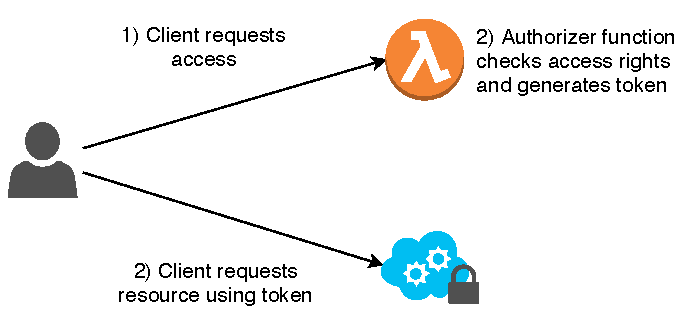
\includegraphics[width=0.6\textwidth]{patterns/valet-key.pdf}
  \caption{Valet Key}
  \label{fig:valetKey}
\end{figure}

\textbf{Solution:} Let the client request an access token from an authorizer function, use the token to directly access a specific resource.

As put forth in section \ref{subsec:thickClient}, serverless function instances do not form long-lived sessions with backend services which means that each service request must be individually authorized. With this in mind, routing client-service requests through a serverless function brings us no apparent security advantage, as both the client and the serverless function are equally untrusted from a service's point of view; on the contrary, having an extra server layer in the middle would only introduce additional latency and cost in data transfer \parencite{adzic2017serverless}. The problem then becomes one of authorizing client-service communication without storing service credentials in the client and thus losing control of service access, and on the other hand without routing each request through the backend and thus in effect paying twice for data transfer.

One authorization pattern that fits the above requirements is the Valet Key. In this pattern the client, when looking to access a resource, first requests access from a special authorizer serverless function. The authorizer function checks the client's access rights and then signs and returns an access token that is both short-lived and tightly restricted to this specific resource and operation. Now for any subsequent calls until token expiration, the client can call the resource directly by using the token as authentication. This removes the need for an intermediate server layer and thus reduces the number of network round-trips and frees up resources. At the same time the pattern avoids leaking credentials outside the authorizer function since the token's cryptographic signature is enough for the resource to validate request authenticity. \parencite{microsoft18cloudPatterns}

The Valet Key relies heavily on cloud services' fine-grained authorization models, as the access token needs to be tightly restricted to a specific set of access permissions; for example read access to a single file in file storage or write access to a single key in a key/value store. Specifying the allowed resources and operations accurately is critical since granting excessive permissions could result in loss of control. Also, extra care should be taken to validate and sanitize all client-uploaded data before use since a client might have either inadvertently or maliciously uploaded invalid content. \parencite{microsoft18cloudPatterns}

\textcite{adzic2017serverless} raise a point about how the Valet Key model of direct client-resource communication can enable significant cost optimization in serverless architectures. For example in case of sending a file to a storage service like AWS S3, having a serverless function in the middle would require a high memory reservation to account for large files as well as paying for function execution time throughout file transfer. As the storage service itself only charges for data transfer, cutting out the middle man and sending files directly from the client reduces costs significantly. The authors emphasize that as FaaS costs ``increase in proportion to maximum reserved memory and processing time [...] any service that does not charge for processing time is a good candidate for such cost shifting''.

\section{Availability patterns} \label{sec:availabilityPatterns}

How to guarantee availability in serverless systems and deal with the platform's performance constraints?

\subsection{Function Warmer} \label{subsec:FunctionWarmer}

\textbf{Problem:} The cold start phenomenon leads to high latency in infrequently invoked functions.

\begin{figure}[h]
  \centering
  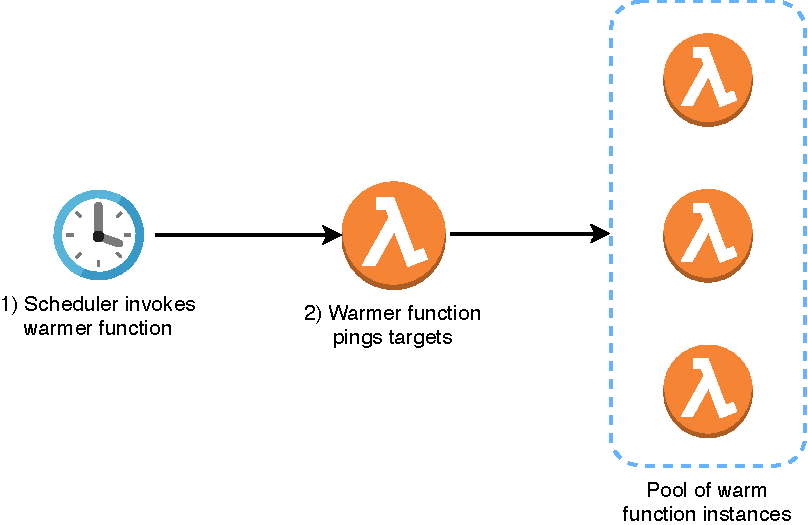
\includegraphics[width=0.65\textwidth]{patterns/function-warmer.pdf}
  \caption{Function Warmer}
  \label{fig:functionWarmer}
\end{figure}

\textbf{Solution:} Ping a function periodically to retain infrastructure and keep the function ``warm''.

Section \ref{sec:limitations} introduced cold starts as a major FaaS pain point. To reiterate, a cold start refers to an infrequently invoked function's start-up latency which results from its infrastructure allocation being deprovisioned after a period of inactivity. \textcite{lloydserverless} for example observed a 15x increase in startup delay for cold starts as opposed to warm starts where existing infrastructure gets reused. While this problem is tied to limitations in current FaaS implementations and can be expected to be mitigated by advances in container technology, cold starts can hamper the adoption of FaaS technology in latency-critical applications.

The Function Warmer tackles the cold start problem by ``pinging'' (invoking) a function periodically with an artificial payload to prevent the FaaS platform from deprovisioning its infrastructure \parencite{leitner18industrialpractice}. In detail, the pattern is implemented with a scheduled function (using the Periodic Invoker \ref{subsec:periodicInvocation} or the State Machine \ref{subsec:stateMachine}) that invokes the target function in predefined intervals. Additionally, the target function's handler is instrumented with logic to handle warming invocations: the handler identifies the artificial payload and replies accordingly without running the whole function. If the aim is to keep several concurrent function instances warm, the Function Warmer should invoke the same function multiple times with delayed executions. Now with the function warmed up and its infrastructure retained, any subsequent invocations can be served with minimal latency.

\textcite{leitner18industrialpractice} note two drawbacks inherent to the pattern: the extra code needed in functions to manage warming invocations, and the invocation cost induced by pinging. The first point is largely a matter of tooling, and indeed many of the FaaS frameworks reviewed by \textcite{kritikos18frameworks} are already equipped to handle pinging logic. As for the latter point, the cost depends on how long the platform retains idling containers for. Investigating infrastructure retention in AWS Lambda, \textcite{lloydserverless} find that host containers are reused when invoked again within 5 minutes; a pinging request in 5 minute intervals then comes down to 8640 invocations per month which is well beyond the free tier offered by most platforms. \textcite{bardsley18optimizationStrategies} likewise note that ``this approach will not significantly raise the cost of the deployment since calls to ping the relevant Lambdas would only have to be made infrequently''. It's also notable that even with the extra pinging costs a FaaS solution can be more economical than a VM-based one: \textcite{lloyd18migration}, while leveraging the Function Warmer to retain a 100 concurrent function instances, observe a ~400\% improvement over cold function performance and a 17.6x reduction in hosting costs compared to VM instances.

A more fundamental issue with the Function Warmer pattern is its necessity in the first place, as ideally the problem of start-up latency would be done away with by the platform. \textcite{leitner18industrialpractice} note that patterns such as the Function Warmer ``can be seen as developers struggling with the inherent limitations of FaaS and working around them''. \textcite{lloydserverless} also point fingers to the platform side, urging cloud providers to ``consider opportunistically retaining infrastructure for longer periods when there is idle capacity to help offset the performance costs of container initialization''. The pattern represents, however, a practical solution to a real limitation that all FaaS platforms suffer from at least for the time being. \textcite{bardsley18optimizationStrategies} similarly conclude that ``whilst this approach somewhat defeats the purpose of a system which should dynamically scale in response to demand it is nevertheless a viable strategy in mitigating the effect of cold Lambdas on overall latency''.

\subsection{Singleton} \label{subsec:Singleton}

\textbf{Problem:} External dependencies like database connections are re-initialized upon each function invocation, leading to degraded performance.

\begin{figure}[h]
  \centering
  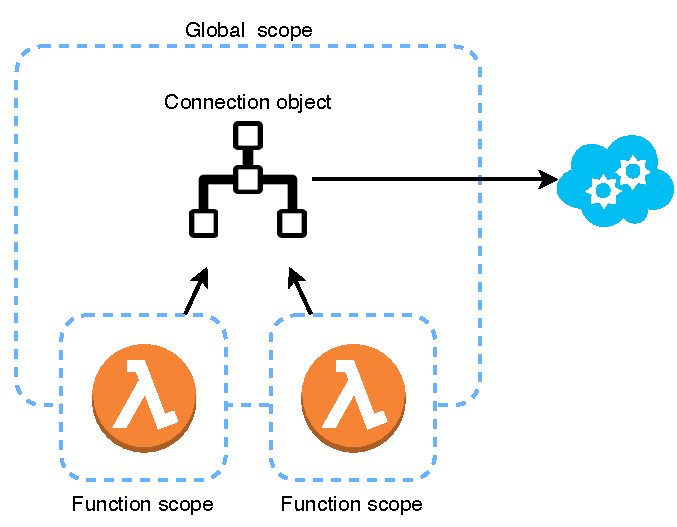
\includegraphics[width=0.55\textwidth]{patterns/singleton.pdf}
  \caption{Singleton}
  \label{fig:singleton}
\end{figure}

\textbf{Solution:} Leverage global scope within your serverless function code to take advantage of container reuse.

Web applications often perform some sort of initialization as a part of their start-up process. Typical examples include connecting to a database and reading configuration or other static objects into runtime memory. In a conventional web application the cost of this initialization phase is negligible as it happens only once in the beginning of a long-running server process. Serverless function instances on the other hand are continuously torn down and recreated, so any delay in initialization has a significant impact on overall performance.

The way containers are reused by FaaS platforms enables us to mitigate the problem. As established earlier in section \ref{sec:limitations}, after a function instance terminates the platform retains its container for a while in case of another invocation. The next function instance, when reusing this ``warm'' container, has access to the runtime variables already initialized during the previous execution. In detail, a reused container retains all of the global or static variables defined outside the function handler (an example of which is presented in listing \ref{lst:handlerExample}). The serverless Singleton pattern consists of reusing these pre-established variables and thus saving us the cost of re-initialization. For example, instead of reconnecting to a database in the beginning of each invocation, a single database connection can be shared by a number of subsequent instances. To implement the Singleton involves declaring such connections and other reusable objects in the global scope and having logic in place to check if a connection already exists before creating a new one. Like its object-oriented namesake \parencite{gamma94designPatterns}, the pattern ensures a single global instance per given resource as well as its ``lazy initialization'' i.e. creation on first use. \parencite{aws18serverlessLens}

\subsection{Bulkhead} \label{subsec:Bulkhead}

\textbf{Problem:} Multiple workflows in a single function leads to a high-latency execution path degrading the others' performance.

\begin{figure}[h]
  \centering
  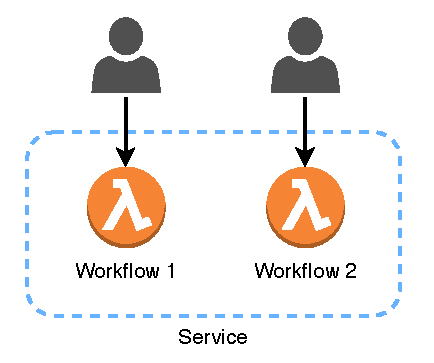
\includegraphics[width=0.35\textwidth]{patterns/bulkhead.pdf}
  \caption{Bulkhead}
  \label{fig:bulkhead}
\end{figure}

\textbf{Solution:} Isolate high-latency code into separate functions to avoid resource contention.

A \textit{bulkhead} refers to a sectioned partition in a ship's hull designed to prevent the whole ship from filling with water and sinking in case of an accident. Similarly in cloud computing context the Bulkhead pattern refers to isolating ``elements of an application into pools so that if one fails, the others will continue to function'' \parencite{microsoft18cloudPatterns}. The idea is to prevent a situation where a single service, when facing resource exhaustion due to a load peak or application error, brings down all of its consumers with it causing a cascading failure and large-scale service interruption. The way this is achieved is by partitioning resources into self-contained blocks divided along lines of expected load and availability requirements: a separate service instance for each consumer, for example, or conversely a separate set of consumer resources (such as threads) for each consumed service \parencite{nygard07releaseIt}. Now even with one service unavailable the system as a whole can deliver some level of functionality.

What are the serverless implications of this inter-service resource contention problem? It seems that FaaS platforms already ensure resource isolation as each function instance runs in its own container. Declaring the problem solved might be premature, however, namely for two reasons: first of all as shown by \textcite{wang18peekingbehindcurtains}, function instances, albeit isolated on a container-level, do suffer from resource contention on a VM level -- a byproduct of some platforms' scheduling strategy of scaling a single function in the same VM. Secondly, a single function can contain multiple execution paths with varying latencies, which can lead to intra-service resource contention. \textcite{bardsley18optimizationStrategies} for example demonstrate customer data function with endpoints for both refreshing a token and simply requesting it: a case
where the ``asymmetrical nature of the performance profile between the refresh and request calls, with the refresh operation suffering significantly higher latency than the request call, could cause refresh calls to unnecessarily divert requests to cold Lambdas''. Put another way, resource contention can occur inside a single FaaS function when an infrequently invoked high-latency workload degrades the performance of a more frequently invoked low-latency one.

While the VM-level resource contention is only addressable by platform providers, the function-level one is mitigated with finer function granularity. A serverless Bulkhead pattern then comes to mean splitting high-latency workflows from a single function into their own functions. In the customer data example above, for example, this required ``separating the request and refresh functionality into separate Lambdas to prevent high latency in one part of the system adversely affecting another'' \parencite{bardsley18optimizationStrategies}. As per \textcite{adzic2017serverless}, the serverless paradigm already does away with economic incentives for bundling applications together in larger deployment units; likewise AWS best practices guide towards ``smaller functions that perform scoped activities'' \parencite{aws18serverlessLens}. As well as helping to avoid resource contention, the Bulkhead enables workflows to scale independently. Maintaining a larger number of functions does still incur an operations overhead, however, and partitioning workflows might not be trivial.

\subsection{Throttler} \label{subsec:throttler}

\textbf{Problem:} A rapidly scaling FaaS function overwhelms a non-scaling downstream service, resulting in function timeout.

\begin{figure}[h]
  \centering
  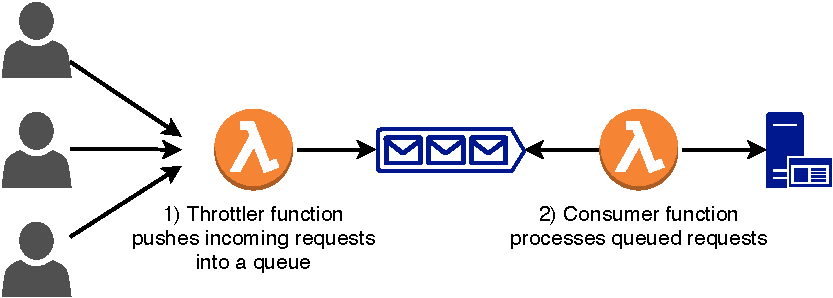
\includegraphics[width=0.7\textwidth]{patterns/throttler.pdf}
  \caption{Throttler}
  \label{fig:throttler}
\end{figure}

\textbf{Solution:} Add a message queue in front of downstream service to throttle bursts of concurrent requests originating from FaaS.

Serverless platforms scale out horizontally in response to increased demand -- up to a 1000 concurrent function instances in case of AWS Lambda \parencite{awslambda0218}. This configuration-free elasticity is a major FaaS selling point and plays well together with similarly autoscaling BaaS services. Scalability can turn into a pitfall, however, when interacting with conventional non-scaling resources, since a rapidly scaling FaaS function has the potential to overwhelm components that lack similar scaling properties or are otherwise not designed to accept high-volume traffic \parencite{cncf18serverlessWG}. This can have the effect of rendering the whole system unavailable by what is essentially a self-inflicted Denial of Service-attack. How would for example an on-premise database with strict connection limits fare with said 1000 concurrent instances? Avoiding non-scaling components in serverless architectures isn't feasible either as few systems have the luxury of not depending on any pre-existing components. Migrating these components into the cloud or deploying enough on-premise hardware to meet peak demand can also be prohibitively costly and organizationally difficult.

Addressing the problem then calls for some mechanism to protect downstream services from intermittent load spikes caused by FaaS scaling. The simplest solution is to apply a limit on the number of concurrent function instances -- a configuration option most FaaS platforms provide. AWS documentation for example states that ``concurrency controls are sometimes necessary to protect specific workloads against service failure as they may not scale as rapidly as Lambda'', particularly in case of ``sensitive backend or integrated systems that may have scaling limitations'' and ``database connection pool restrictions such as a relational database, which may impose concurrent limits'' \parencite{aws18serverlessLens}. While managing to ease the pressure on downstream services, this solution causes non-responsivity in consuming applications and arguably fails to take full advantage of the FaaS platform.

The Throttler represents a more sophisticated approach, based on buffering the bursts of concurrent requests originating from FaaS and resolving them asynchronously in a more controlled pace. A serverless adaptation of the Queue-Based Load Leveling cloud design pattern \parencite{microsoft18cloudPatterns}, the Throttler adds a message queue between the function and the downstream service so that upon a new request, instead of immediately invoking the service and waiting for a reply, the function pushes the request into the queue and responds to the consumer with an acknowledgement of receipt. It's then the job of another function to consume the queue and resolve service requests. By adjusting queue consumption rate, request spikes can be resolved in a smoother thus avoiding service resource exhaustion and function timeouts. A persistent queue also provides a further level of robustness as requests are not lost even in case of service outage.

\textcite{baldini17currentTrends} utilize the Throttler to ``control the flow of data between two services'' in a hypothetical issue tracking system, further improving on the queue consumer's network efficiency by implementing batching. \textcite{rotem12soa} in turn presents an equivalent SOA pattern, the Decoupled Invocation: ``acknowledge receipt at the service edge, put the request on a reliable queue, and then load-balance and prioritize the handler components that read from the queue''. The pattern helps with the coupling and performance bottleneck problems of request-reply communication but comes with the downside of latency. Also since message queues are a one-way communication mechanism, it may be necessary to utilize a pattern like the Event Processor (section \ref{subsec:Eventprocessing}) for the consumer to access the actual service response. Finally, the Throttler can be seen analogous to the Service Activator EIP pattern which consists of adding a messaging layer (the queue and its consumer function in our case) in front of a synchronous service to turn it into an asynchronous one \parencite{hohpe2004enterprise}.

\subsection{Circuit Breaker} \label{subsec:circuitBreaker}

\textbf{Problem:} A non-responsive third-party service causes accumulating FaaS charges as a function needlessly performs and waits for requests that time out.

\begin{figure}[h]
  \centering
  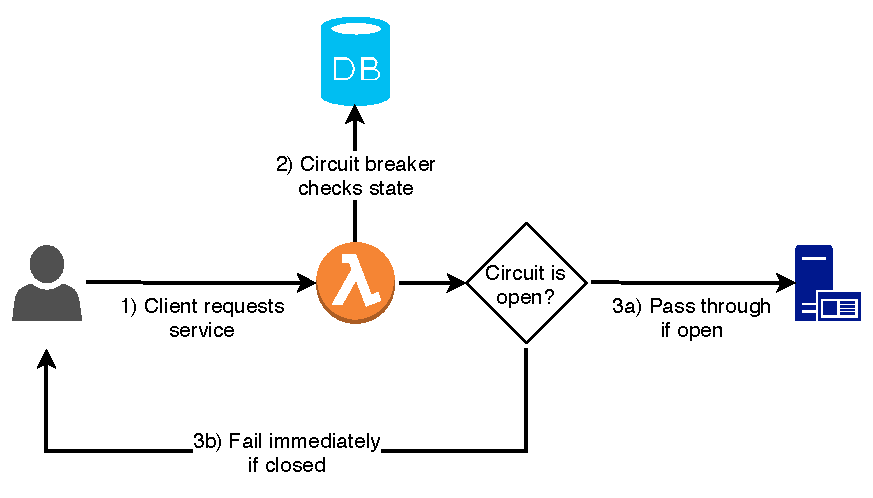
\includegraphics[width=0.73\textwidth]{patterns/circuit-breaker.pdf}
  \caption{Circuit Breaker}
  \label{fig:circuitBreaker}
\end{figure}

\textbf{Solution:} Restrict service access in times of degraded operation to reduce service load and prevent performing operations that are likely to fail.

Transient network errors and temporary service unavailability are common and unavoidable occurrences in distributed systems. A simple request retry mechanism is usually enough for the system to recover from such temporary interruptions, but unexpected events -- human error, hardware failure etc. -- can occasionally lead to much longer downtime \parencite{microsoft18cloudPatterns}. In these cases request retry becomes less valid of a strategy, leading instead to wasted consumer resources and latency in error handling. Furthermore, a large number of consumers bombarding an unresponsive service with repeated requests can end up exhausting service resources and thus inadvertently prevent recovery. These points are particularly relevant for serverless consumers where the pay-as-you-go pricing model means that waiting for timeouts directly translates into extra costs. A serverless consumer's scaling properties also make it more prone to service exhaustion: as a consumer takes longer to execute while waiting for timeout, the platform ends up spawning more concurrent consumer instances which in turn tie up more service resources in a spiraling effect. As observed by \textcite{bardsley18optimizationStrategies}, ``it is in situations like this that retry is not beneficial and may well have harmful effects if it ends up spinning up many cold Lambdas''.

Instead of re-execution we're then looking to prevent calling an unresponsive service in the first place. The Circuit Breaker pattern, as popularized by \textcite{nygard07releaseIt}, does just that ``by wrapping dangerous operations with a component that can circumvent calls when the system is not healthy''. Akin to an electrical circuit, the pattern keeps track of requests passing through it and in case an error threshold is reached it momentarily blocks all requests. In closer detail, the Circuit Breaker operates either in \textit{closed}, \textit{open} or \textit{half-open} mode. In times of normal operation the circuit is closed, i.e. requests get proxied to the service as usual. When the service becomes unresponsive and the number of error requests exceeds a threshold the circuit breaker trips and opens the circuit, after which service requests fail immediately without attempts to actually perform the operation. After a while when the service has had a change to recover, the circuit goes into half-open mode, passing through the next few requests. If these requests fail, the circuit trips open and again waits for a while before the next try; if they succeed, the circuit is closed and regains normal operation. Via this mechanism the Circuit Breaker benefits both the consumer and the service, as the consumer avoids waiting on timeouts and the service avoids being swamped by requests in times of degraded operation.

As a stateful pattern the Circuit Breaker needs to keep track of circuit mode, number of errors and elapsed timeout period. A serverless implementation can utilize either the Externalized State (section \ref{subsec:externalizedState}) or State Machine (section \ref{subsec:stateMachine}) pattern for managing this information. Additionally, the pattern can be implemented either alongside an existing consumer or as its own function between a consumer and a service similarly to the Proxy pattern (section \ref{subsec:proxy}). As to further implementation details, \textcite{nygard07releaseIt} notes it is important to choose the right error criteria for tripping the circuit and that ``changes in a circuit breaker’s state should always be logged, and the current state should be exposed for querying and monitoring''. Instead of returning a plain error message the open circuit can also implement a fallback strategy of returning some cached value or directing the request to another service. An open circuit could even record requests and replay them when the service regains operation \parencite{microsoft18cloudPatterns}.

The Circuit Breaker is similar to the SOA pattern of Service Watchdog \parencite{rotem12soa} in the sense that both implement self-healing by means of restricted service access. What differentiates the two is who's responsible: the Service Watchdog depends on an integrated component inside the service to monitor its state whereas the Circuit Breaker only acts external to the service, on the basis of failed requests. This distinction makes the Circuit Breaker easier to deploy against black-box components.
